\documentclass{article}

\usepackage[a4paper, margin=2cm]{geometry}

\usepackage[utf8]{inputenc}
\usepackage[czech]{babel}
\usepackage{fvextra}
\usepackage{csquotes}
\usepackage{expl3}

\usepackage{parskip}
\usepackage[hidelinks, unicode, pdfusetitle]{hyperref}

\usepackage{float}
\usepackage{minted}
\usepackage{graphicx}
\usepackage{xcolor}
\graphicspath{{images}}

\title{34-3-4 Horňáci a Dolňáci}
\author{Benjamin Swart}

\begin{document}

\maketitle

\section{Zadání}

Máme za úkol najít hranu, jejímž odstraněním získáme graf, který lze obarvit dvěmi barvami - třeba červenou a modrou.

Graf je možné obarvit dvěmi barvami právě tehdy, když v něm nejsou žádné cykly s lichou délkou. Snažíme se tedy najít nějakou hranu, která leží na všech takových cyklech.

\section{Hledání cyklu}
\label{section:cycle}

Zvolíme si libovolný vrchol a obravíme ho červeně. Poté z něj spustíme nějaký druh prohledávání - jestli do hlouby nebo do šířky je docela jedno. Ke každému vrcholu si uložíme, ze kterého vrcholu jsme se na něj dostali, a obarvíme ho opačnou barvou od barvy jeho \enquote{rodiče}. Jakmile nějaký vrchol obarvíme stejnou barvou jako nějakého z jeho sousedů můžeme prohledávání ukončit.

\begin{figure}[H]
    \centering
    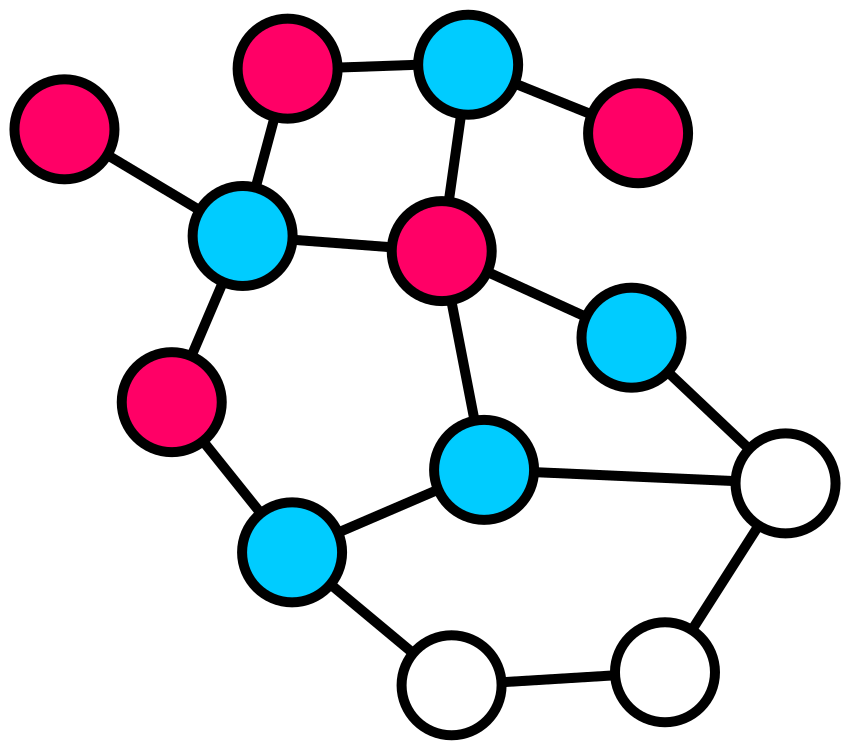
\includegraphics[height=5cm]{graph/colored.pdf}
\end{figure}

Z obou stejně obarvených vrcholů budeme procházet odkazy na rodiče dokud se nedostaneme do kořene grafu. Sepíšeme odkazy na všechny vrcholy, které podkáme včetně začátku a konce. Z obou seznamů škrtámě první prvky, dokud jsou v obou seznamech stejné. Nakonec spojíme poslední společný prvek, první seznam a druhý seznam pozpátku. Nyní máme seznam vrcholů, které po řadě tvoří cyklus s lichým počtem prvků. Hledená hrana určitě leží na tomto cyklu. Seznam si uložíme a navíc si ke všem vrcholům uložíme umístění v tomto seznamu, abychom mohli rychle určit vzdálenost mezi libovolnými dvěmi vrcholy v tomto cyklu.

\begin{figure}[H]
    \centering
    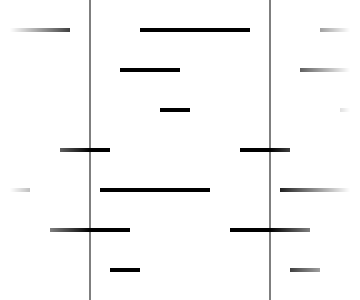
\includegraphics[height=6cm]{cycle/empty.pdf}
\end{figure}

\section{Tvorba intervalů}
\label{section:interval-construction}

Vytvoříme si seznam vrcholů sousedících s cyklem.

Vybereme libovolného souseda a obarvíme ho červeně. Spustíme z něj obarvovací vyhledávání jako v části \ref{section:cycle}, akorát si nemusíme pamatovat rodiče. Na vrcholy v cyklu vstupovat nebudeme. Zapamatujeme si však všechny právě obarvené vrcholy, které s cyklem sousedí. Pokud narazíme na obarvovací anomálii, tak vstup nemá řešení.

\begin{figure}[H]
    \centering
    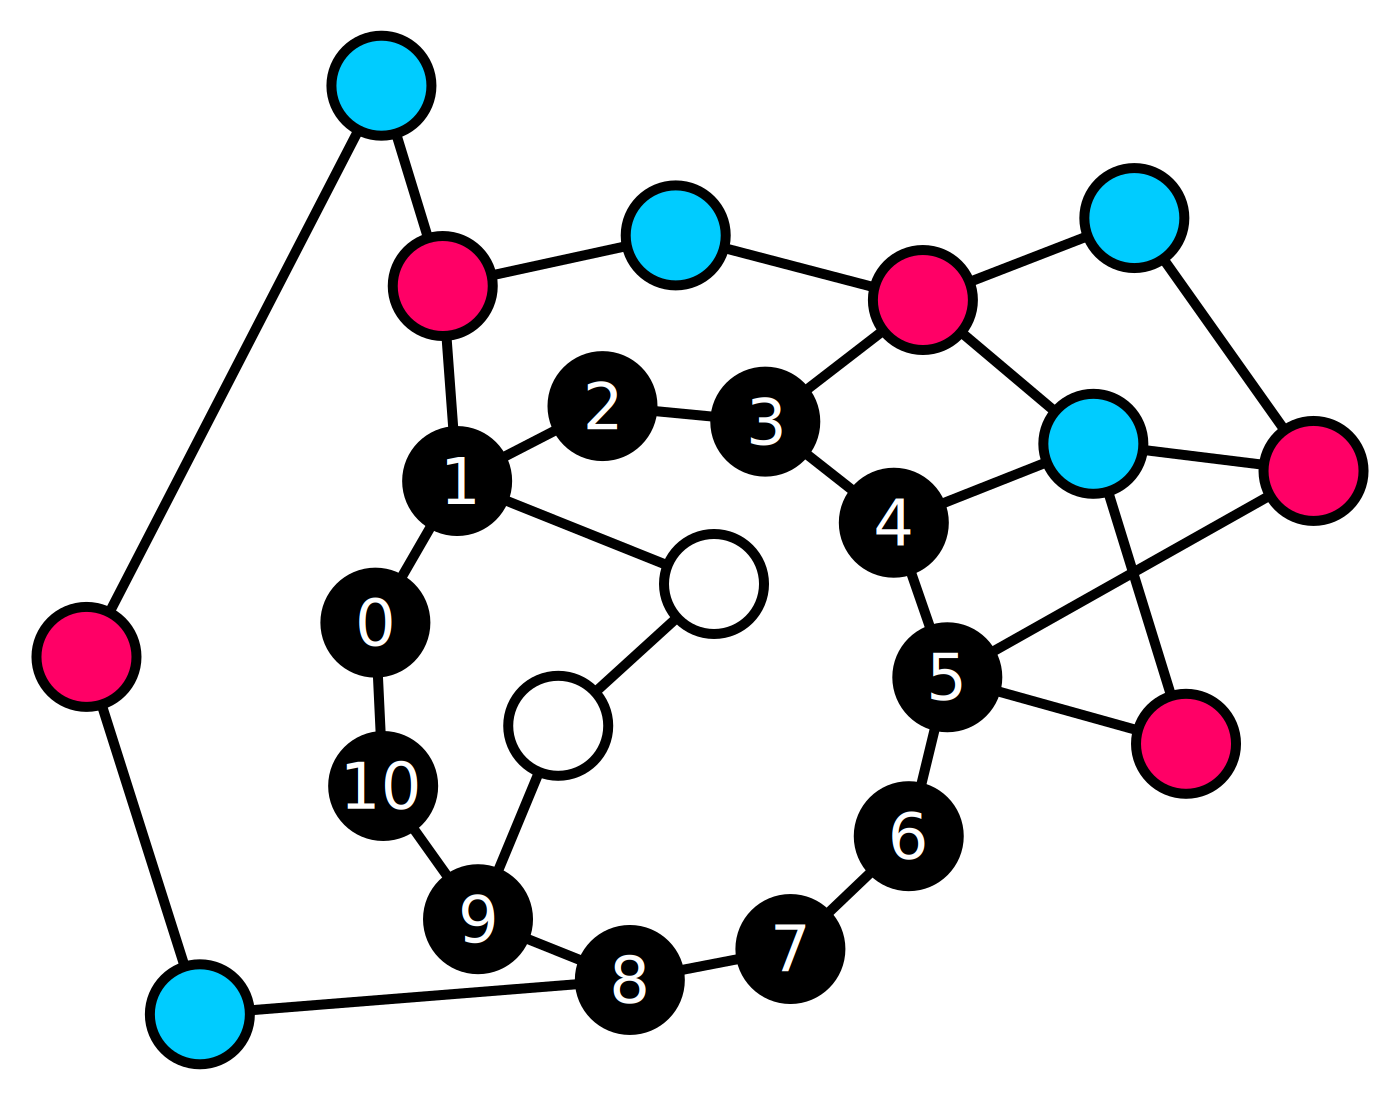
\includegraphics[height=6cm]{cycle/first.pdf}
\end{figure}

Právě obarvené sousedy seřadíme podle čísla vrcholu v cyklu, se kterým sousedí. Pokud jeden vrchol sousedí s více vrcholy v cyklu, tak ho do grafu umístíme dvakrát. Stačí nám si pamatovat jeho barvu. Pokud jeden vrchol v cyklu sousedí s více právě obarvenými vrcholy, tak logicky musí mít stejnou barvu. Uložíme ji jen jednou.

Nyní máme seznam, který vypadá takto:

\begin{enumerate}
    \item \textcolor{red}{1}
    \item \textcolor{red}{3}
    \item \textcolor{blue}{4}
    \item \textcolor{red}{5}
    \item \textcolor{blue}{8}
\end{enumerate}

Vytvoříme z něj seznam intervalů:

\begin{enumerate}
    \item \textcolor{red}{1} -- \textcolor{red}{3}
    \item \textcolor{red}{3} -- \textcolor{blue}{4}
    \item \textcolor{blue}{4} -- \textcolor{red}{5}
    \item \textcolor{red}{5} -- \textcolor{blue}{8}
    \item \textcolor{blue}{8} -- \textcolor{red}{1}
\end{enumerate}

Tyto intervaly projdeme. Pro každý vypočítáme vzdálenost druhého vrcholu od prvního a zkontrolujeme, jestli je lichá nebo sudá. Pokud je vzdálenost mezi vrcholy sudá a jejich barva je různá, tak našli jsme našli smyčku o liché délce. Hledaná hrana tedy musí ležet v tomto intervalu. Pokud je vzdálenost mezi vrcholy lichá a jejich barva je stejná, tak jsme rovněž našli anomálii a hrana musí v tomto intervalu ležet. Pokud je však vzdálenost sudá a barvy stejné nebo vzdálenost lichá a barvy různé, tak v tomto intervalu anomálie neleží. Problematickou smyčku jsme však našli stejně. Pokud je šířka intervalu \((a,b)\) sudá, je šírka intervalu \((b,a)\) nutně lichá a naopak. Hledaná hrana tedy v tomto intervalu určitě neleží.

Z logiky věci najdeme jen jeden interval, o kterém víme, že v něm hrana lěží. Ten si uložíme do seznamu a pokračujeme s dalším sousedem cyklu, kterého jsme ještě neobarvili. Toto opakujeme dokud nám sousedé nedojdou.

\begin{figure}[H]
    \centering
    \includegraphics[height=6cm]{cycle/second.pdf}
\end{figure}

\section{Průnik intervalů}

Ze sekce \ref{section:interval-construction} máme seznam otevřených intervalů v cyklické množině vrcholů, na kterých určitě leží hledaná hrana. Tento seznam může vypadat například takto:

\begin{enumerate}
    \item 4 -- 7
    \item 9 -- 6
    \item 5 -- 9
\end{enumerate}

Zbývá jen najít nějakou hranu v jejich průniku.

Budeme procházet všechny hrany a vyhodnocovat, jestli leží v průniku všech intervalů. Abychom to mohli snadno posoudit, přepracujeme výše uvedený seznam v seřazený seznam událostí:

\begin{enumerate}
    \item[4.] Začátek intervalu
    \item[5.] Začátek intervalu
    \item[6.] Konec intervalu
    \item[7.] Konec intervalu
    \item[9.] Konec intervalu
    \item[9.] Začátek intervalu
\end{enumerate}

Tento seznam je seřazen primárně podle čísla vrcholu kterému událost náleží, sekundárně konce před začátky.

Také si přímočarým průchodem seznamu spočítáme, v kolika intervalech leží hrana 0 -- 1. Tento počet si uložíme do proměnné.

Nyní budeme postupně zpracovávat události ze seznamu. Vždy nastavíme aktuální hranu na \(t\) --- \(t+1\), kde \(t\) je čas události. Následně snížíme nebo zvýšíme počet intervalů, ve kterých se hrana nachází. Pokud se tento počet rovná celkovému počtu intervalů, tak hranu vypíšeme a program ukončíme.

\section{Složitost}

Většina kroků tohoto algoritmu běží v \(O(n)\), jen potřebná řazení běží v \(O(n * log(n))\). Paměťová složitost je \(O(n)\), ukládáme jen podmnožiny a jednoduché transformace vstupních dat.

\end{document}